\documentclass[border=10pt]{standalone}
\usepackage[svgnames]{xcolor}
\usepackage{amsmath}
\usepackage{pgfplots}
\pgfplotsset{compat=newest}
\usepackage[sfdefault]{FiraSans}
\usepackage{FiraMono}
\renewcommand*\familydefault{\sfdefault}
\begin{document}
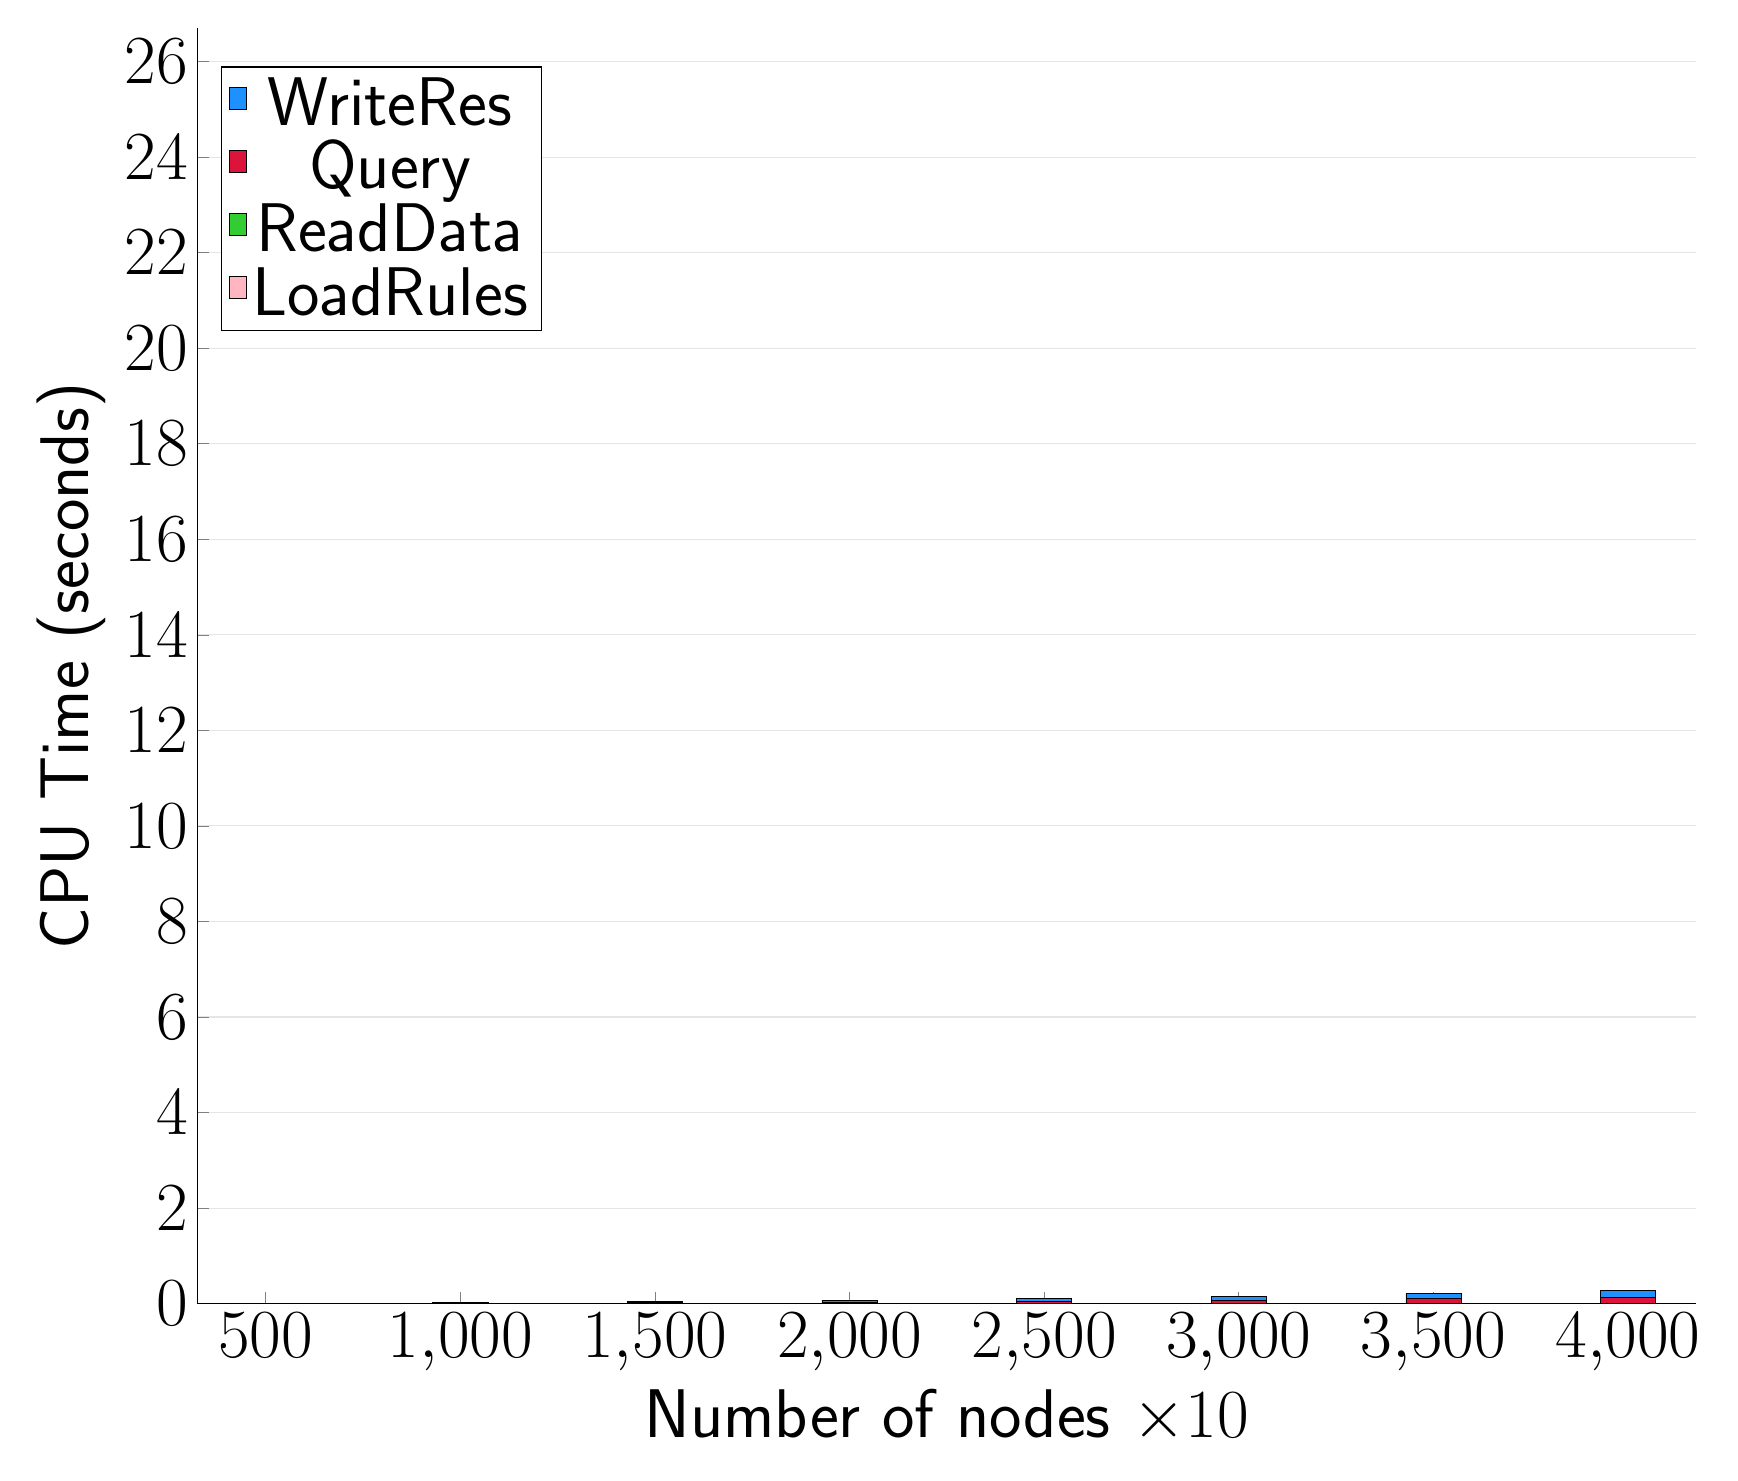
\begin{tikzpicture}
\begin{axis}[
   ybar stacked,
   width=1.7\textwidth,
   bar width=0.7cm,
   ymajorgrids, tick align=inside,
   major grid style={draw=gray!20},
   xtick=data,
   ymin=0, ymax=26.698890000000002,
   axis x line*=bottom,
   axis y line*=left,
   enlarge x limits=0.05,
   legend style={
       at={(0.23, 0.97)},
       anchor=north east,
       legend columns=1,
       font=\Huge,
   },
   ylabel={CPU Time (seconds)},
   xlabel={Number of nodes $\times 10$},
   label style={font=\Huge},
   tick label style={font=\Huge},
]
\addlegendimage{fill=DodgerBlue, draw=black, line width=0.2pt}
\addlegendentry{WriteRes}
\addlegendimage{fill=Crimson, draw=black, line width=0.2pt}
\addlegendentry{Query}
\addlegendimage{fill=LimeGreen, draw=black, line width=0.2pt}
\addlegendentry{ReadData}
\addlegendimage{fill=LightPink, draw=black, line width=0.2pt}
\addlegendentry{LoadRules}
\addplot +[fill=LightPink, draw=black, line width=0.2pt] coordinates {
(500, 0.0006253)
(1000, 0.0006136)
(1500, 0.0006001000000000002)
(2000, 0.000606)
(2500, 0.0006076000000000001)
(3000, 0.0006142999999999999)
(3500, 0.0006074000000000003)
(4000, 0.0006166999999999996)
};
\addplot +[fill=LimeGreen, draw=black, line width=0.2pt] coordinates {
(500, 0.0006023999999999995)
(1000, 0.0010711)
(1500, 0.0015419000000000001)
(2000, 0.0020320999999999994)
(2500, 0.0025322000000000005)
(3000, 0.0030338000000000006)
(3500, 0.003508700000000001)
(4000, 0.0039737999999999996)
};
\addplot +[fill=Crimson, draw=black, line width=0.2pt] coordinates {
(500, 0.0018156)
(1000, 0.007549499999999999)
(1500, 0.0179535)
(2000, 0.03140049999999999)
(2500, 0.048666)
(3000, 0.0712826)
(3500, 0.0981746)
(4000, 0.1285222)
};
\addplot +[fill=DodgerBlue, draw=black, line width=0.2pt] coordinates {
(500, 0.0022570000000000003)
(1000, 0.009241200000000001)
(1500, 0.0205551)
(2000, 0.036341500000000006)
(2500, 0.05707829999999999)
(3000, 0.0808805)
(3500, 0.1121383)
(4000, 0.14042190000000002)
};
\end{axis}
\end{tikzpicture}

\end{document}
